\chapter{An Approach to Intention-oriented Organizational Modeling}
\label{chap:approach}
This chapter describes in detail about the technical approach that has been taken to solve the problem mentioned in problem statement Section \ref{sec:problemstatement} of Chapter \ref{chap:introduction} and to satisfy all of the requirements mentioned in the Section \ref{sec:requirementssupoorting} of Chapter \ref{chap:analysis}. The first section of this chapter provides an overview of the intention-oriented organizational modeling process approach. The second section discusses in detail second phase (P2) of the InProXec method, i.e., Model Informal Processes. The third section discusses in detail about the \textit{top-down approach}, which helps to realize the intention-oriented organizational modeling. The fourth section discusses the design methodology followed to realize this approach of developing a descriptive modeling web based editor. The final section discusses in detail about the relationship between each entity types of this approach. 

%%%%%%%%%%%%%%%%%%%%%%%%%%%%%%%%%%%%%%%%%%%%%%%%%%%%%%%%%%%%%%%%%%%%%%%%%
\section{Overview of the Modeling Process}
\label{sec:overviewmodelingprocess}
%%%%%%%%%%%%%%%%%%%%%%%%%%%%%%%%%%%%%%%%%%%%%%%%%%%%%%%%%%%%%%%%%%%%%%%%%
The main focus of this approach is to develop a web-based modeling tool which can be used by business experts to model the informal processes, intentions, strategies and capabilities. Also in this thesis work, the scope of modeling is limited only to the descriptive type of modeling i.e., models that describe processes declaratively by providing only information about what has to be done. As we mentioned before, the resource definitions required for the editor is made available from the first phase P1 of the InProXec approach. Business experts develop descriptive models through the editor using these resource models to achieve main intention that contains sub-intentions, strategies etc. The reason for following descriptive modeling approach is due to the fact that models reuse descriptive data and these stored models provides means of execution for the phases P3 and P4 of InProXec. The model provides necessary concepts and relations for modeling the core elements of resource-centric organizational modeling. Resources are abstract description which are made concrete during initialization of an instance. There are also resource specific views based on the participating resources' role. For example, based on the privilege provided to a participant he can view/edit/own/follow the instances. Initializing resource-centric models requires \textit{acquiring} and engaging interrelated resources \cite{Sungur2015} which is explained in a detailed way in the following sections of this chapter. 

%%%%%%%%%%%%%%%%%%%%%%%%%%%%%%%%%%%%%%%%%%%%%%%%%%%%%%%%%%%%%%%%%%%%%%%%%
\section{Second Phase of InProcXec - Model Informal Process}
\label{sec:informalprocessmodeling}
%%%%%%%%%%%%%%%%%%%%%%%%%%%%%%%%%%%%%%%%%%%%%%%%%%%%%%%%%%%%%%%%%%%%%%%%%
This approach of Informal Process Modeling is directed towards modeling the informal process based on their intentions rather than their activities. This is due to the fact that intentions only define \textit{what to do} rather than \textit{how to do}. Since this phase is part of InProXec method, the properties and requirements described in previous approaches \cite{Sungur2014a,Sungur2015} also applies to informal process modeling phase. The developed system serves as an holistic web based editor to create, view and update all the associated entities of informal process like intentions, capabilities, strategies etc., along with informal process. Also from our detailed explanation in previous sections about the importance of resources in organizational modeling  and along with the fact that phase P2 receives resource defintions as input from phase P1 of InProXec method we can apprehend that resource definitions are the lowest level in the hierarchy of resource-centric organizational modeling approach. The sequence of steps to be carried out using the developed editor has been shown in the Figure  \ref{fig:processdiagram}. It is important to note that in the figure, only solid round edged rectangles are part of the developed editor. The tasks to be carried out in each of the steps in developed editor is described as below:

\begin{figure}
	\centering
	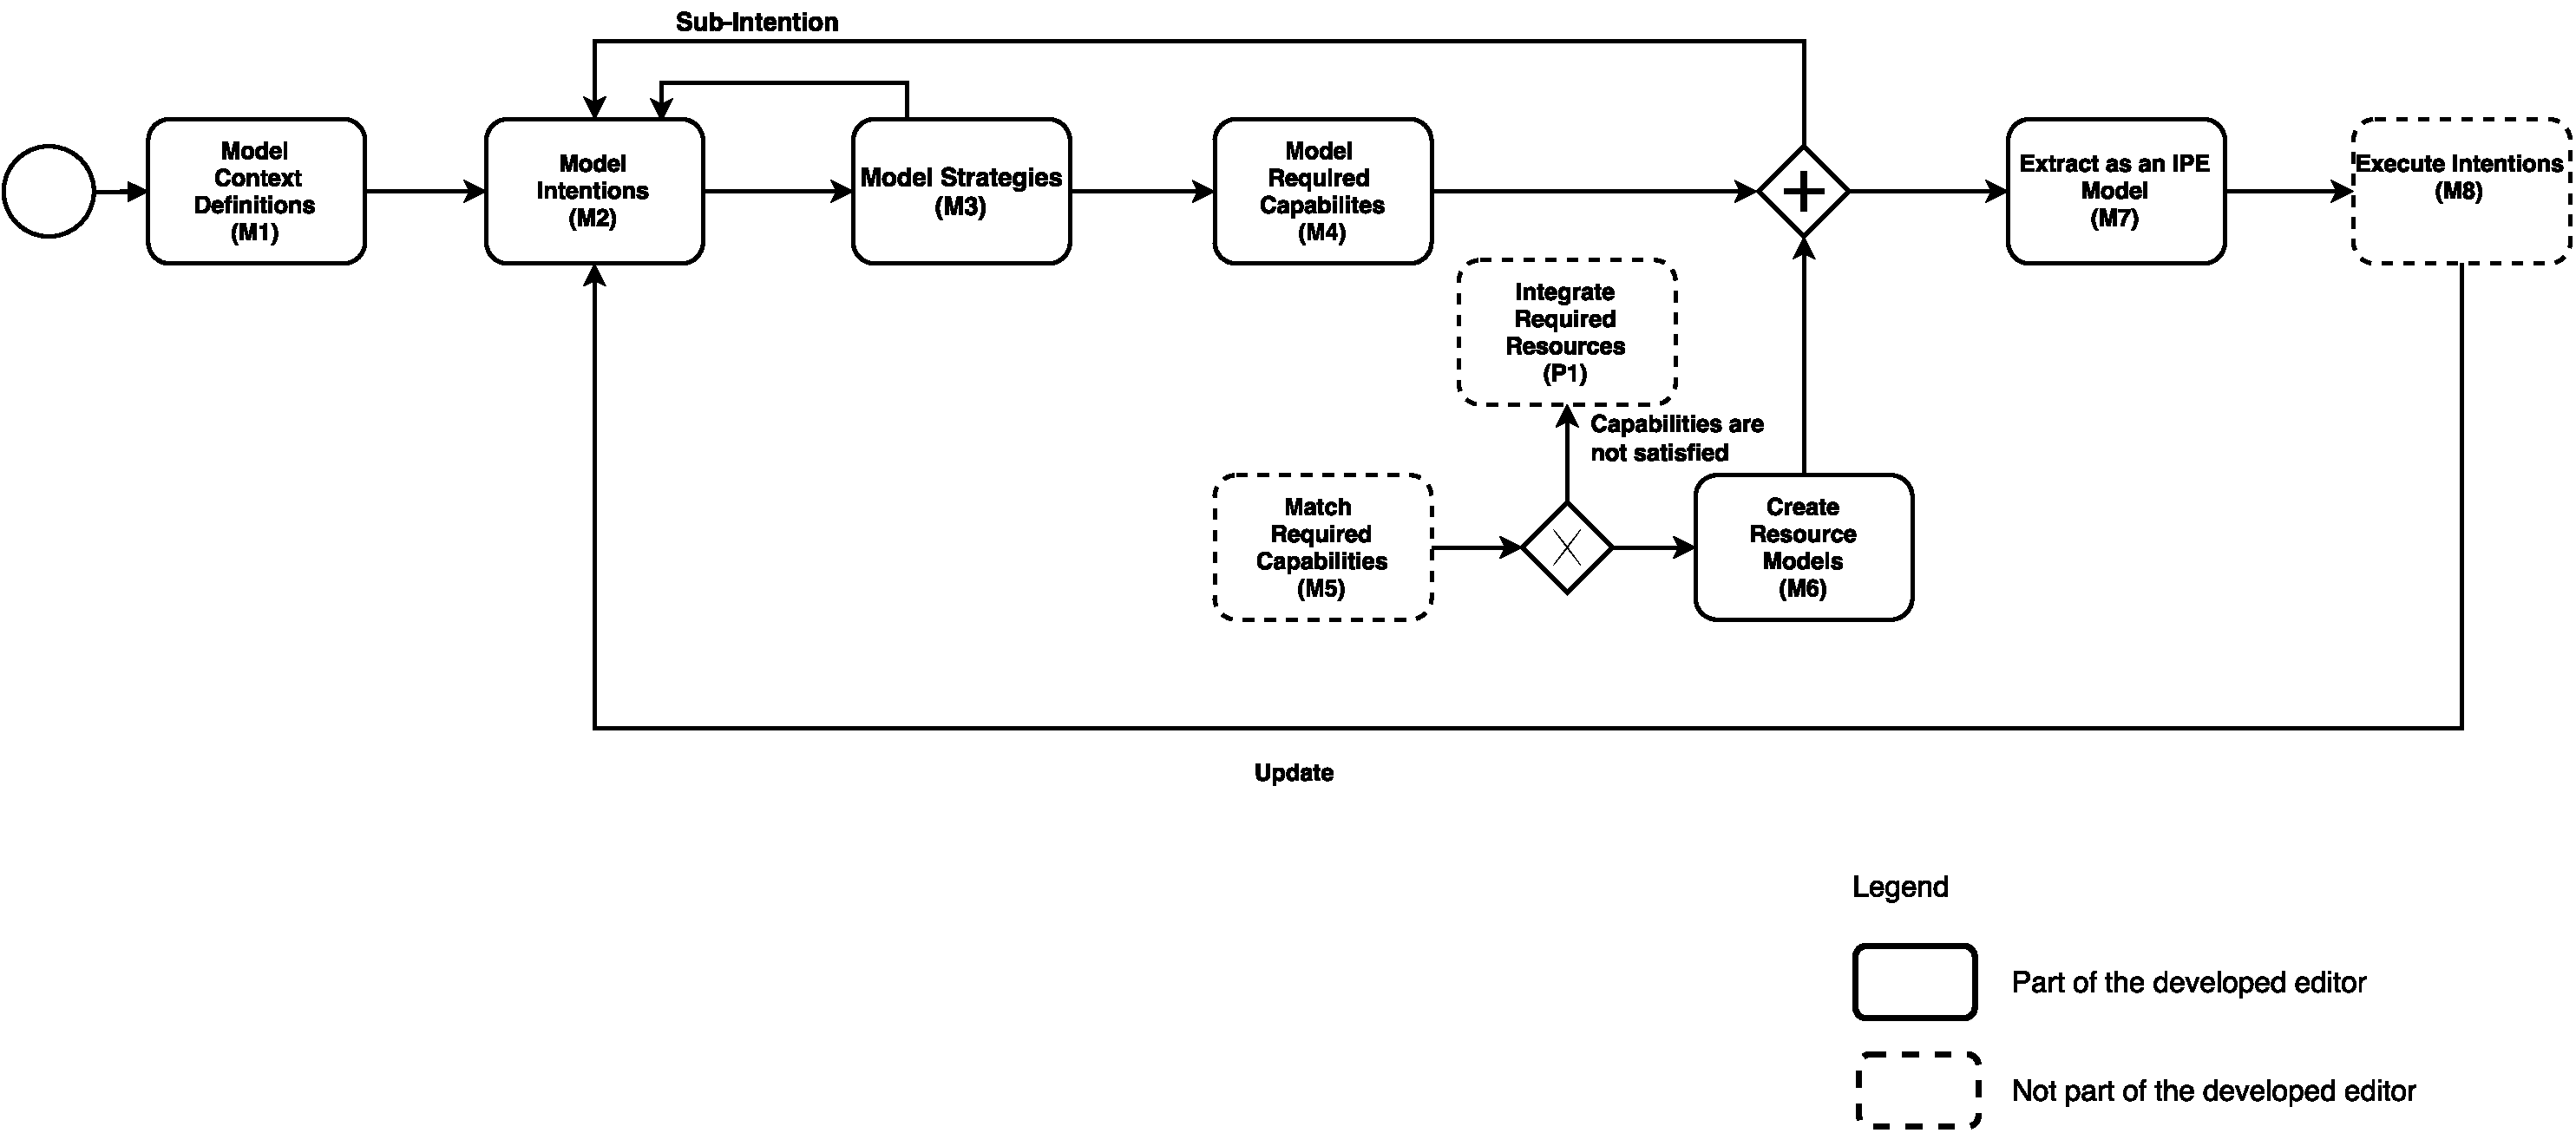
\includegraphics[width = \textwidth]{processmodeling.pdf}
	\caption{Steps of the Informal Process Modeling}
	\label{fig:processdiagram}
\end{figure}

\subsubsection{Model Context Definitions (M1)}  
The first step is to model context definitions, where we can model both basic properties like name and namespace of a context definition and entity specific properties like contained contexts, entity definitions etc., of a context definition.  

\subsubsection{Model Intentions (M2)}  
Similar to context definition modeling (M1), the second step (M2) is to model intentions. The context definitions created in step M1 can be used to specify initial and final contexts of an intention. Intentions can contain sub-intentions and contradicting intentions. These type of sub intentions and contradicting intentions are also modeled as intentions in this step and their type of relation to specific intention are mentioned. Intentions are defined hierarchically, which can contain and extend sub-intentions.It is depicted by a double circle in organizational notations. The sub-intentions are refined starting from main intentions. Intentions are associated with strategies.

\subsubsection{Model Strategies (M3)}  
Once intentions are identified and modeled, the third step is modeling of strategy to achieve a specific intention. As mentioned earlier in Section \ref{sec:entitytypesrepresentation}, an intention can have multiple strategies.  A  strategy is a method or plan chosen to bring  desired results, such as achievement of an intention or solution to a problem. Strategies are associated with capabilities. 

\subsubsection{Model Required Capabilities (M4)}  
After modeling of strategies, capabilities required to achieve an intention in a specific strategy is modeled. A strategy can require multiple capabilities which has been explained in detail with a suitable example in the following Chapter \ref{chap:motivatingScenario}. 
A capability is the ability to provide business values like software applications, resources and potential of the actor to make decisions even in changing situations \cite{Stirna2012}. Capability describes the ability provided by a resource or required by an intention. The performers of an informal process should posses certain skills and roles to achieve the intention. These type of required skills are modeled during this step.

\subsubsection{Create Resource Models (M6)}  
After matching the resources and capabilities i.e after finding the correct resource that has the capability to carry out the process, the resource models are created. The need for modeling a new intention may arise in parallel during modeling of resources. This has been explained with a suitable example in the following Chapter \ref{chap:motivatingScenario}.  A resource can be a people or tool those/that drive towards the successful execution of the process. It is key for achieving specified process intentions. In the context of this work, the definition of organizational resources refers not only the entities that are capable of doing work but also entities that have an impact on the outcome of the processes, e.g., software tools, human performers, data etc.      

\subsubsection{Extract as an IPE Model (M7)}  
After the completion of above mentioned steps, the modeled entities can be extracted as an IPE model which can be reused. 

The other steps denoted in dashed round edged rectangle are not part of developed web editor. The steps are matching of required organizational capabilities (M5) that are satisfied by resource models and integration of required resources (P1). If there is no suitable matching capability then phase P1 of InProXec can be carried out again until a matching capability is found. If Capabilites are satisfied resource models can be created. The created resource models(M6) along with modeled capabilities can be extracted as an IPE Model(M7) which will be provided as input for the next step execution of intentions (M8). After the execution of an intention, the status of an intention is updated inside the specific intentions's property. 

%%%%%%%%%%%%%%%%%%%%%%%%%%%%%%%%%%%%%%%%%%%%%%%%%%%%%%%%%%%%%%%%%%%%%%%%%
\section{A Top-down Modeling Approach}
\label{sec:topdownapproach}
%%%%%%%%%%%%%%%%%%%%%%%%%%%%%%%%%%%%%%%%%%%%%%%%%%%%%%%%%%%%%%%%%%%%%%%%%
Intentions are defined hierarchically, intentions can contain and extend intentions. Intentions can contradict to itself as well. Intentions are associated with strategies, thus intentions can be realized through strategies. Strategies are associated with capabilities. These capabilities are of two types \textit{functional capabilities} and \textit{cross functional capabilities}. Functional capabilities are associated with resources and cross functional capabilities are associated with functional capabilities. Each informal process model is a strategy that has capabilities, strategies, resources that are created out of capabilities and intentions. In the Figure \ref{fig:topdownapproach}, it has been shown that how this modeling approach starts modeling from top level of the hierarchy and does modeling until the lower level is reached. 

\begin{figure}
	\centering
	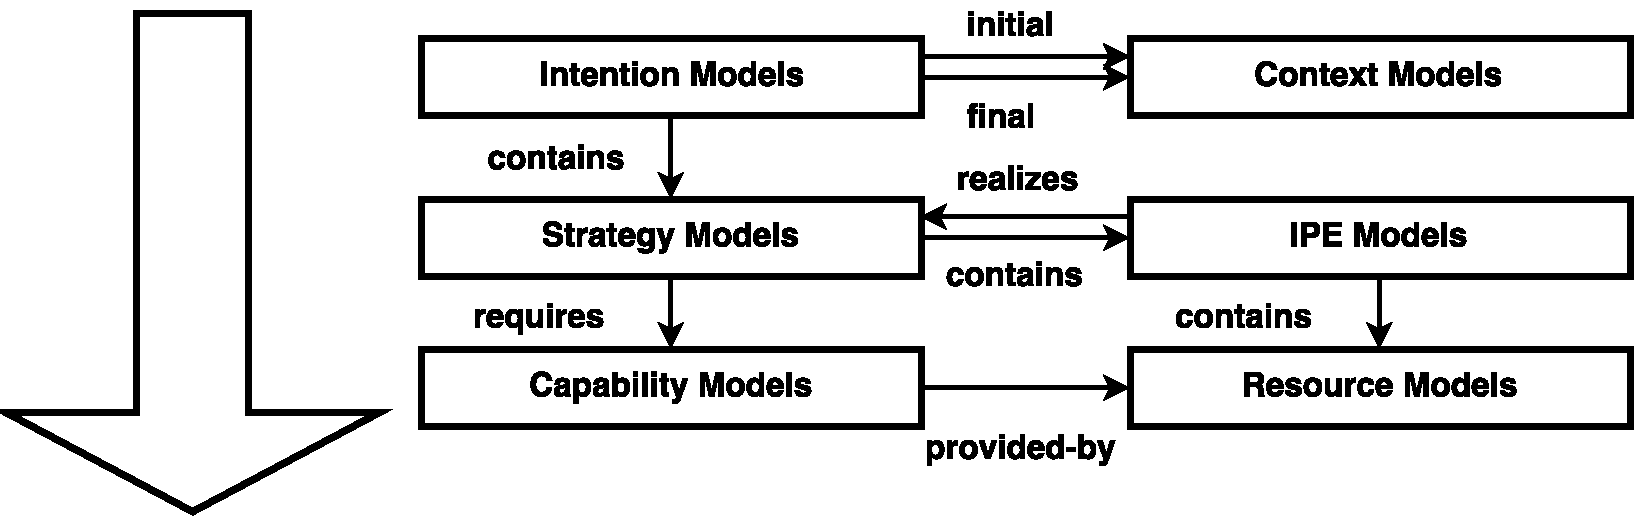
\includegraphics[width=\textwidth]{TopDownApproach.pdf}
	\caption{Intention-oriented Organizational Modeling: A Top down Modeling Approach}
	\label{fig:topdownapproach}
\end{figure}

Bider et al \cite{bider2005strategy} propose a strategy-driven modeling approach of processes. Processes are defined based on the goals and refinement continues until meaningful operation level is reached. Consequently, created models are easily changeable as they are decoupled from their operational terms. Such declarative approaches provide more flexibility and enable easier change of the business process models \cite{Sungur2016}. As we mentioned before, the modeling approach in our context is descriptive modeling approach which starts from the top level and refines modeling until the bottom level is reached. 

%%%%%%%%%%%%%%%%%%%%%%%%%%%%%%%%%%%%%%%%%%%%%%%%%%%%%%%%%%%%%%%%%%%%%%%%%
\section{Design Methodology}
\label{sec:designmethodology}
%%%%%%%%%%%%%%%%%%%%%%%%%%%%%%%%%%%%%%%%%%%%%%%%%%%%%%%%%%%%%%%%%%%%%%%%%
When designing the user interface components and functionalities required to develop the tool, most of the similar functionalities are 
designed as common functionalities and re-used. This reduced unnecessary functional redundancies and overhead. The common functionality methodology are followed for both model functions and view functions.  Some of the important methodologies followed with respect to user interface components design are 1. multiple items to be selected from multiple list items are displayed as  \textit{list group} 2. selecting single item from multiple items are displayed as \textit{drop down}. For example, to select multiple strategies from a list of strategies, available strategies are displayed as a list from which the user can select desired number of strategies. Another important methodology followed during user interface design is, for every entity the properties should be displayed only under the respective properties tab. For example, in the Figure \ref{fig:samplescreen}, the basic properties such as name, target namespace and process type of an informal process model should be displayed only under the respective basic properties tab and similarly for all other tabs. This methodology is followed uniformly throughout the design of all the entity types such as intention definitions, strategy definitions, capability defintions, context definitions, instance definitions and informal process definitions and for all of their property types. 

All data are stored only under the data artifact. This applies to the labels and text fields of all user interface elements and this data can be updated only through the handler function. Through \textit{settings} option, the user can add new namespace and intention relation type. From the Figure \ref{fig:samplescreen}, it is clear that a standard design methodology has been followed to display the list of available entity types such as intentions, strategies, capabilities etc., and to display their respective properties such as basic, entity specific, instance data, etc., properties. Though the top-down modeling approach \ref{sec:topdownapproach}, shows that definition of each entity type is contained within another entity type, as per the user interface design, separate entities references each other using the unique reference identifier but does not contain all properties of referenced entity. For instance, a strategy containing an intention should contain only the intention's unique reference identifier but not the actual intention itself. Later, in the view of strategy, actual intention properties are fetched and displayed based on the unique reference identifier. 

\begin{figure}
	\centering
	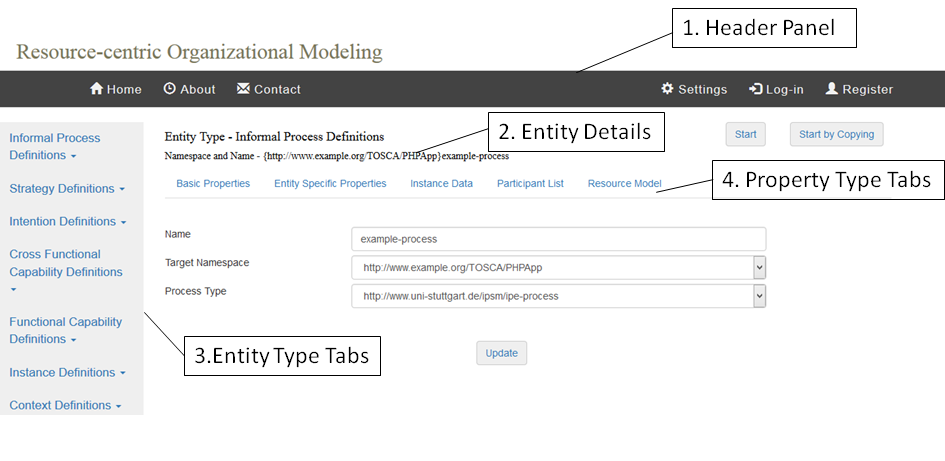
\includegraphics[width=\textwidth,angle=0]{samplescreen.png}
	\caption{User Interface Design of the Editor}
	\label{fig:samplescreen}
\end{figure}

The research objectives mentioned in Chapter \ref{chap:introduction} are also met during the development of the editor. The validity of the research objectives are discussed in Chapter \ref{chap:casestudy} using the motivating scenario discussed in Chapter \ref{chap:motivatingScenario}. The methodology followed to satisfy the requirements are detailed below.

\textit{Organizational intentions transparency} (R1): In the current functioning system, users are stored in database artifact and these users can login through their valid credentials. Thus the logged in user can view the intention and its associated entities.

\textit{Organizational intention resource-based cost estimation} (R2): Intentions are associated with strategies, which are associated with capabilities and hence with resources. Cost is calculated in a recursive manner. For example, consider we need to calculate cost of an instance whose entity type is intention. To calculate the cost we go recursively to the lower levels starting from the required level. Since our instance is of type intention, we start iterating through every associated strategy, and for each associated strategy, we iterate through their instances as well. In case the cost of an instance of a strategy has not been specified, we specify it by calculating the cost of instances of associated informal process definitions. For informal process definitions, we use the cost resource definitions. This ends the recursion and returns the total sum as the cost of an instance, of type intention

\textit{Organizational intention achievability estimation} (R3): Similar to resource-based cost estimation for an intention, the achievability of an intention also depends on its instance state. For example, if an instance of type intention is associated with a strategy which also has an instance that is completed. Then the total number instances remaining to be completed to achieve an intention is calculated as one out two instances. 

\textit{Intention oriented working style} (R4): The users can login and create intention models, strategy models, informal process models etc., through the developed editor. 

\textit{Participative organizational modeling} (R5): Each entity type that can be acquired or instantiated has list of participants with their corresponding privileges. 

\textit{Re-use of organizational knowledge} (R6): The descriptive information about each models can be stored and their changes are also updated. 
 
